\chapter{Gamification in Software Engineering Education:
An Empirical Study}
\label{ch:gamificationExperiment}

This chapter describes our experience and provides an evaluation of the adoption of gamification in a 60-hour introductory course on Software Engineering at Federal University of Minas Gerais (UFMG), in Brazil, during the second semester of 2016. This course covers a plethora of topics, from requirements engineering to software design, implementation, and testing. The classes were attended by 36 undergraduate students in Computer Science and Information Systems. We introduced two elements of games, namely badges and leaderboards, to engage students and promote a safe competition environment by rewarding students for their achievements. While badges award students by specific achievements, a leaderboard aims to indicate the overall performance of every student with respect to their peers. We introduced these game elements using the course webpage, where students could have regular feedback. 

We evaluated the proposed course features in two steps. First, we applied a survey to 18 volunteer students to collect their feedback about the impact of badges and leaderboards during their course experience. Second, we interviewed six randomly selected students for a deeper investigation about their perceptions about the course and the use of game elements. Our results show that badges had a greater impact on the motivation of students than leaderboards. In addition, we observed that students would like to see badges more frequently in other courses. On the other hand, leaderboards had poor appraisals from the students in the survey. However, interviews revealed that students used periodic reports on their partial grades for comparing their performance against other students, which is similar to a leaderboard. A general complaint is that students feel that the most appropriate reward for their performance is extra grades rather than achievement recognition. Despite the number of participants interviewed, the focus of this study is to report our experiences and observations, rather than validating hypothesis.

The remainder of this chapter is organized as follows. Section II provides the necessary theoretical foundation for the study. Section III describes the gamification elements introduced in the Software Engineering course under investigation. In Section IV, we describe the design of this study. Section V presents the results of the study. In Section VI, we discuss our findings regarding the research questions defined for this study. Section VII discuss the threats to the validity of the study while we discuss the related work in Section VIII. Section IX concludes this research paper

\section{Course setup}

Every year at Federal University of Minas Gerais (UFMG) in Brazil, about 100 students take a face-to-face Software Engineering course. The introductory Software Engineering course (“SE Course”, henceforth) aims to introduce students to the concepts and methods required for the development of large software intensive systems. Its prerequisite is familiarity with object-oriented programming, demonstrated through a successful completion of the Modular Programming course at UFMG (or equivalent course in another university).

This Software Engineering course is mainly based on two textbooks: Software Engineering by Sommerville [14] and The UML User Guide by Booch, Rumbaugh, Jacobson [15]. The course syllabus includes: software development process, agile methods, software requirements analysis and specification, software design, system implementation and testing, software reuse, and software quality.
Previous instances of this course had already been the target of experimental studies on alternative educational methods [16] [17]. In the second semester of 2016, we planned the inclusion of gamified elements in the course format. Specifically, we adopted badges and leaderboards. A badge is a common element in games to recognize specific achievements of players. Leaderboard is recurring element in games to foster competition, allowing players to compare their progress or performance against other players. Both elements capitalize on principles of social status and reputation.

In the context of the SE Course, we used badges to recognize specific actions of students. We established eight badges in this first iteration of a gamified course. Examples of badges are listed below.

•	Agility and Precision: Awarded to the student who first submitted a correct solution for a specific practical task, such as, code implementations, or homework, or practical assignment.

•	Clean Code: Awarded to the student who used code standards explained in the classroom to document the code and keep it easy to read.

•	Performance Improvement: Awarded to the student who had the greater improvement in grade from the first to the second exam.

•	Online Participation: Awarded to the students who accessed all online material of this course. 

In the first day of class, the instructors communicated students about the existence of badges, but they did not provide details on how to obtain them. Whenever a student met the criteria to receive a badge, all students were communicated in the classroom and the badge was revealed in the course website with the name of students who obtained it. Table I shows examples of badges awarded to students during the course. Additionally, these badges did not provide direct bonus grades or any advantage in the course, apart from achievement recognition. However, the attendance to the badges criteria would positively contribute to a better performance on the course assignments and activities.

TABLE I. 	EXAMPLES OF FOUR BADGES IN THE SE COURSE

Leaderboard was incorporated with two resources: (i) a chart with partial grades and (ii) a Hall of Fame. The chart with partial grades was a digital document that was updated periodically and accessible in the course website, where students could track their grades and compare their performance against other students. To preserve the anonymity, the students were identified only by their university registration number. The “Hall of Fame”, on the other hand, is a special page in the course website that acknowledges the names of the top three best students of each course semester and the top ten students of all time. 

TABLE II. 	TOP TEN STUDENTS OF ALL TIME IN THE SE COURSE

Table II shows the Hall of Fame with the top-10 best grades of all time in the SE course. The second column of this table indicates the student grade in 100 points. The third and fourth columns indicate the semester and the student name, respectively. Although Figure 2 presents the best scores since 2012, this table was only made available in the second semester of 2016 based on historical data.

\section{Study settings}

This section explains how we planned and executed this study. Section IV-A presents the study goal and research questions while Section IV-B discusses the research method we adopted. Section IV-C presents the survey and Section IV-D explains the structure of an interview with 6 randomly selected students.

\subsection{Study Goals and Research Questions}

The goal of this study is to investigate how the use of gamification could contribute to motivate students in Software Engineering education. To achieve this goal, we formulated two Research Questions (RQ) presented below.

\textbf{RQ1.} What are the student perceptions on the use of badges in the SE Course?

\textbf{RQ2.} What are the student perceptions on the use of leaderboards in the SE Course?

\subsection{Study Design and research methods}

To answer the research questions, we adopted two techniques. First, we conducted a survey with the students to collect general impressions of the course (Phase I). Second, we conducted interviews to further understand the perception of the students about the gamification techniques used in the course (Phase II).

For both phases, the target population was all 36 students enrolled in the SE Course. They were invited to participate in both studies by e-mail. To reduce possible bias, one of the authors, who was not directly involved in the course execution, was responsible for the invitation of participants and data collection. The students were instructed that the participation in the survey and in the interviews was not compulsory and this participation did not provide any benefits in grades. Besides that, the student names were not revealed to the course instructors during the data analysis, to ensure that students would not be embarrassed for giving negative responses.

\subsection{Planning of the Study Phase I - Survey}

Survey is an empirical strategy for collecting information from or about people to describe, compare or explain their knowledge, attitudes, and behavior using questionnaire or checklist [18]. In the first phase of our study, a survey was applied to collect a quantitative perspective of the students’ perception on the use of badges and leaderboards in the SE course. 

We created a questionnaire on Google Forms  with two parts: the first one was composed of 4 questions about the background of the students; the second part had 8 questions about the perception of the students about the gamification elements used in the course. Table III shows the list of questions in the first part of our survey and Table IV summarizes the questions of the second part. The background questions were named BQ1 to BQ4, while the questions of the second part of our survey were named SQ1 to SQ8. Tables III and IV describe the possible answers for each question. Invitations were sent by e-mail to all 36 students formally enrolled in the course, as described in Section IV-B.

TABLE III. 	SURVEY QUESTIONS ON THE PARTICIPANT BACKGROUND

TABLE IV. 	SURVEY QUESTIONS ON THE PARTICIPANT PERCEPTION OF THE GAMIFICATION ELEMENTS  IN THE SE COURSE

\subsection{Planning of the Study Phase II - Interviews}

An interview is a research method defined by a conversation where questions are asked and answers are given [19]. In this study, we used interviews to compliment and deepen the results observed in the survey (Phase I), providing a qualitative perspective on the students’ perception of the gamification elements introduced in the SE Course.

As described in Section IV-B, we sent invitation e-mails to all 36 students formally enrolled in the course. In the invitation email, we made it clear that the participant would have their personal data kept anonymously. We interviewed participants individually, face-to-face or by video-conference, as they prefer in order to make the situation more comfortable and natural for them. The interviews were executed after the conclusion of the course, and that the course instructor would not have access to the names of the participants, to reduce possible bias. Table V describes the interview script. This script is composed of 9 questions, named IQ1 to IQ9. For instance, the first question (IQ1 in Table V) asks students if they track their partial grades during the course.

TABLE V. 	INTERVIEW QUESTIONS

\section{Results}

In this section, we discuss the results of the study. Section 
V-A presents the descriptive analysis of the results from the survey (Phase I). In Section V-B, we discuss the qualitative results of the interviews (Phase II).

\subsection{Study Phase I - Survey Results}

From the 36 students in the SE course, 18 participants answered the survey. Of these students, 17 were undergraduate students of the Information System course and only 1 was an undergraduate student in the course of Computer Science. 

Figure \ref{fig:gamificationbq} presents the results for the background questions BQ1 to BQ3 regarding the background of the participants. The first question (BQ1) was about the participant familiarity with the term “gamification”. 11 participants (61.1\%) answered that they were familiar with this term (8 were somewhat familiar and 3 were definitely familiar). Only 4 participants (22.2\%) claimed that they were definitely not familiar with the term. Our second question (BQ2) was about the frequency in which participants play games. 6 participants (33.3\%) claimed that they play games every day, 4 participants (22.2\%) play few times a week and 5 participants (27.7\%) play sometimes a month. Only 3 participants (16.6\%) claimed they play games only few times a year. No participant claimed that never plays games. In the third question (BQ3), we inquired the participants about their appreciation for games. The results show that most of participants (13 – 72.2\%) confirmed that they like playing games.

\begin{figure}[!h]%th
\centering
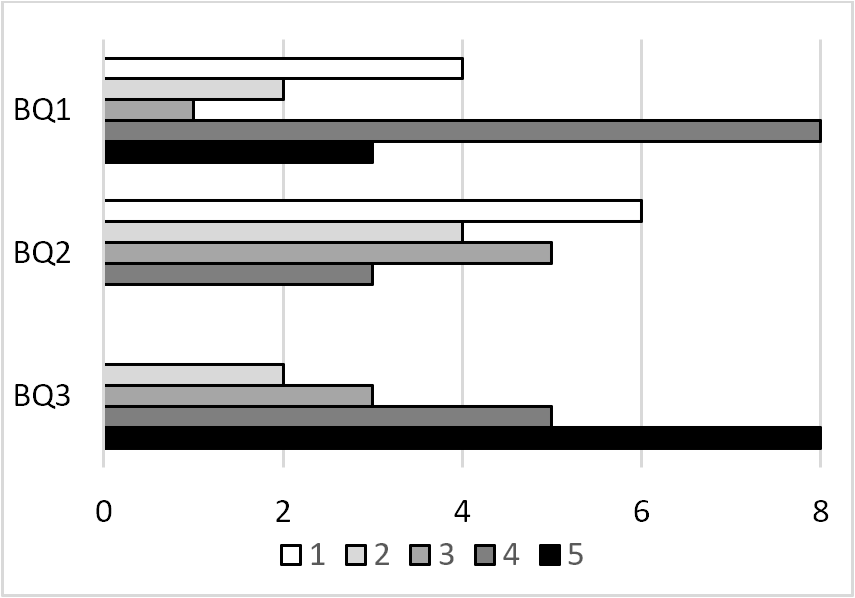
\includegraphics[width = 0.5\textwidth]{img/gamificationBQ.png}
\caption{Results for the survey background questions BQ1 to BQ3.}
\label{fig:gamificationbq}
\end{figure}

Figure \ref{fig:gamificationbq4} shows the results for the last background question (BQ4) in this pre-questionnaire. BQ4 aims to understand the reasons why the participants like playing games. In total, 17 participants (94.4\%) stated that they aim to have fun. In addition, 12 participants (66.6\%) claimed that one reason is to develop skills and the same number of students said they like to face challenges when play games. Less frequently, 11 participants (61.1\%) aimed to enjoy spare time and 8 participants (44.4\%) aimed for competition.

\begin{figure}[!h]%th
\centering
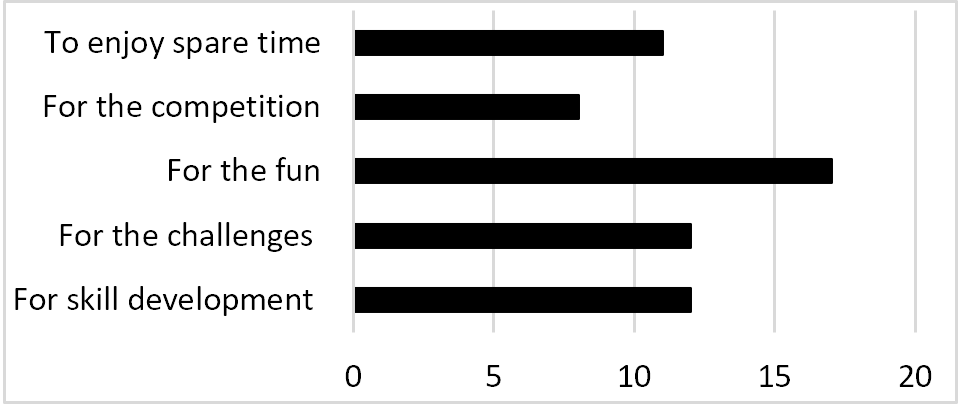
\includegraphics[width = 0.7\textwidth]{img/gamificationBQ4.png}
\caption{Results for the survey background question BQ4.}
\label{fig:gamificationbq4}
\end{figure}

Figure \ref{fig:gamificationsq14} presents the responses on the perception of students about the gamification elements introduced in the course. Questions SQ1 to SQ4 (described in Section IV-C) were defined to investigate the students’ perception on the implementation of badges in the course. 

As described in Section III, eight badges were implemented in the SE course. When asked if the participants found relevant the use of badges (SQ1), the responses were slightly positive (i.e., 7 positive, 6 neutral, and 5 negative responses as presented in Figure 3). However, when asked if these badges motivated them towards a better performance in the course (SQ2), Figure 3 shows that the responses were negative (9 negative, 5 neutral, and 4 positive responses). When asked if they would appreciate the existence of more badges in the course (SQ3), or the existence of similar resource in other courses (SQ4), the responses were positive in both cases. These data are indications that badges were well received by students, but they were not seen as a key factor of motivation by the majority of them. Further investigation about these results was explored in the interviews.

\begin{figure}[!h]%th
\centering
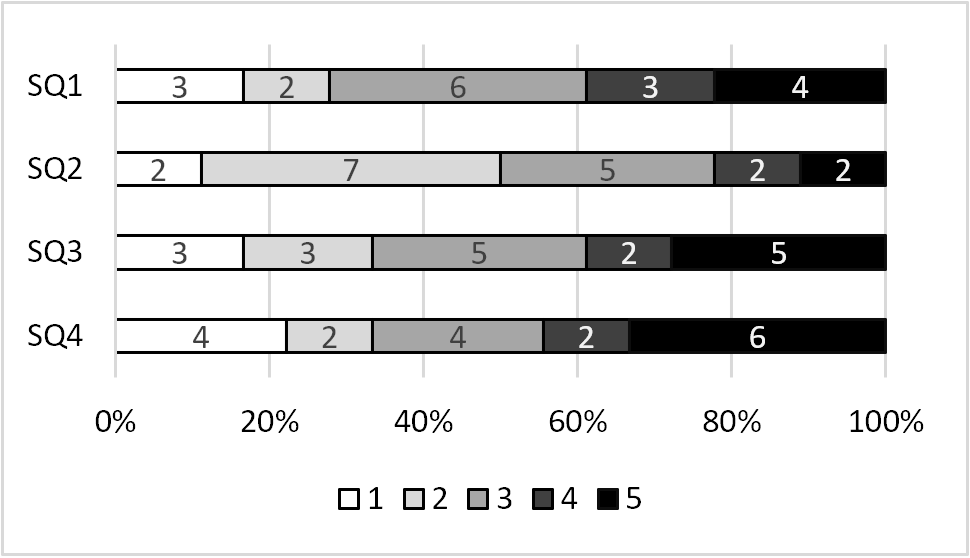
\includegraphics[width = 0.6\textwidth]{img/gamificationSQ14.png}
\caption{Survey results on the students perception on the use of badges.}
\label{fig:gamificationsq14}
\end{figure}

Regarding the leaderboards, specifically the “Hall of Fame”, the survey results were generally negative, as seen in Figure Figure \ref{fig:gamificationsq14}. The questions SQ5 to SQ7 inquired participants about the relevance of such resource (SQ5), about how it motivated them to achieve better performance in the course (SQ6), and about the relevance of such resource in other courses (SQ7). Although there were very positive responses for the three questions, the negative responses were dominant. In the Phase II of this study, we investigated the reasons of such negative perception.

\begin{figure}[!h]%th
\centering
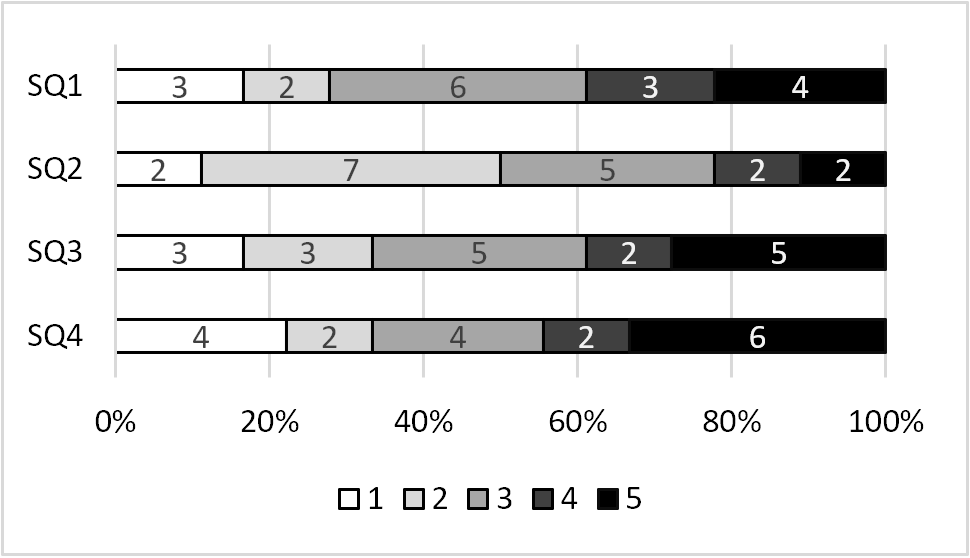
\includegraphics[width = 0.6\textwidth]{img/gamificationSQ14.png}
\caption{Survey results on the students perception of the “Hall of Fame”.}
\label{fig:gamificationsq57}
\end{figure}


Finally, we received 8 responses for the open question SQ8, regarding suggestions and criticism on the use of the game elements introduced in the SE course. Two participants suggested the addition of more badges as transcribed below.

“There should be more badges throughout the course”

“In general, I always work hard on the courses I'm enrolled. Thus, in the Software Engineering course I felt that my dedication was recognized. However, there should be more badges in the course for different types of activities in order to try to reach as many students as possible. In my opinion, the students who have also worked hard, but have not earned any badges, could be discouraged and feel that their effort was not recognized.”

Three participants suggested that badges could be converted to bonus grades:

It was not mentioned by the professor whether anyone who won badges or appeared in the 'Hall of Fame' would earn more grades for this. If I knew this could happen, I would be more motivated.”

“Badges could be converted into extra grades. In my opinion, perhaps it is the only way to really motivate students.”

“(…) Why there are no awards in grades? (…)”

Five students suggested that the course instructor should provide more details on how to obtain the badges, so students could pursue them actively:

“Maybe knowing what badges I could have obtained, it would make me motivated to "work" to get them. We did not have much incentive.”

 “I think if we knew the titles or how to get some badges, we could be more competitive to get them. Since we did not know which badges could be won, it was difficult to focus on something specific in order to earn them. It would be interesting to get at least some badges for the students in the next course. Of course, they could have some ‘extras’ grades. But if the students knew that it was possible to win the 'Clean Code' badges, for example, more students would try to make a better code. The proposal is super interesting.”

“It would be interesting to report about the badges, at the beginning of the course, so students could know about it in advance. And, what are the criteria for choosing the badges; it is also interesting to know. In this course, we had the badge 'Clean Code', for example, what would be 'Clean Code'? What are the specific characteristics the code should have, so that it is chosen? I believe that extra information would be interesting to add to knowledge for students who could not win the badges.”

“It would be interesting to disclosure the activities and rules to earn badges. Thus, we could work focusing on them since the beginning of the course.”

 “This method could be more interesting if the means of evaluation were clearer and more objective. As 'Online Participation', which online actions are rewarded? Log in every day at the platform (online course), or see all classes or post questions? In which case would any of these actions be more accounted than another? Is the ordering for better online participation updated every week? What do you get with your name in badge list or Hall of Fame? Are there awards in grades? Is it visibility among colleagues? And, is it the visibility among colleagues positive?”

\subsection{Study Phase II – Interviews Results}

Based on the results of the survey, we planned and conducted interviews to obtain a better understanding on the student perception on the gamification elements used. Six students accepted the invitation for interviews. The interviews followed the script described in Section IV-D. In order to identify the interviewee responses, we adopt the identifiers “Participant A”, “Participant B”, “Participant C”, “Participant D”, “Participant E”, and “Participant F” to refer to the participants, while preserving their anonymity.

Regarding the leaderboards, we first investigated how students used the information about their progress that we provided. As described in Section III, the leaderboards were introduced in the course with two resources: (i) a chart with partial grades updated regularly, where students could compare their progress against other students; and (ii) a hall of fame. First, we investigated if the students kept track of their progress (IQ1) and if they used the partial grades to compare their performance against their colleagues (IQ2). Except for the Participant A, all participants stated they tracked their progress in the course. Moreover, all participants, except for the participant C stated they used the grade chart to compare their performance against their colleagues. Participant B, Participant D, Participant E, and Participant F stated that it was useful to understand the overall performance of the classmates in order to know what their real performance was. Participant A stated that this comparison was a consequence of the competitiveness in the classroom. However, Participant C claimed that he always tried to achieve the best grades, and it was not interested in comparing their performance to the others.

Regarding the positive aspects of this comparison (IQ3), we observed three main positive feedbacks: (i) students with lower performance than the average performance of the class would feel motivated to perform better, (ii) students try to understand how they could improve their learning strategy, and (iii) they talk to classmates with better performance to exchange knowledge. One possible issue pointed by the participants was the risk of students acting only in response to the general performance of the class, i.e., if everyone is getting poor grades, there is no reason to try to perform better. Participant D also warned about the risk of creating ego conflicts in the class. With respect to motivation of improving because of this comparison (IQ4), only Participant A and Participant D had negative responses. Participant A would only feel inclined to try to perform better in case the class has a better performance in general.
Question IQ5 inquired the participants about their opinion on the “Hall of Fame” resource. Participant A did not like the strategy to implement the Hall of Fame, and claimed that it did not capture the essence of Software Engineering, and it would be better to acknowledge other aspects such as the best product developed instead of grades. The other participants had positive perceptions about the recognition provided by the Hall of Fame.

From the six participants in this study phase, only one (Participant C) received badges (two) during the course. Participant C found the experience positive and rewarding. Even without receiving badges, Participant B, Participant D, and Participant F found this element rewarding and benefic as a form of recognition for specific actions. Except for Participant A, all others responded question IQ7 positively.

When we asked participants about the strategy of not revealing the criteria for receiving each badge, the opinions were mixed. Participants B, C, and E defended the idea of specifying the criteria for each badge as soon as possible, because students would establish additional goals besides the grades and, from an educational perspective, it would become an opportunity to pay attention to aspects that they would not normally observe. For Participants C, D, F, the criteria for obtaining badges could make students focus too much attention on the game aspect and, somehow, they could have a counterproductive effect on learning. Except for Participant A, all students were positive when asked if they would like to see more badges in the course.

\section{Discussion}

This section discusses the results presented in Section V and our general findings regarding the research questions defined in Section IV-A.

\subsection{Badges in a Software Engineering course (RQ1)}

Our results showed a general positive perception of the students towards the use of badges during the course. Considering that we did not explore this resource to the full potential, by having only eight badges, the students showed interest on them.

Student perception on the role of badges was twofold: (i) they served as a social reward, a public recognition of the student skill or effort; and (ii) they served as a secondary goal, besides the grades and approval, to strive for when performing the course activities. These two elements can be further explored to motivate students not only in performing better in the course, but also as a motivation to further explore Software Engineering good practices. For instance, it can make students aware of good practices related to the use of tools, of good practices for coding, and so on. In this initial study, we opted for keeping the requirements for earning badges in secret to avoid the students expectative of grades, but we are aware of the motivation it can generate.

One of the students participating in the interviews was particularly unsatisfied about the gamification elements in the course, because he wanted they to explore the practical nature of Software Engineering and professional practices. We are considering this feedback for further improvements of the SE course. However, in general, the results showed that the positive impressions about the use of badges were greater than the negative ones.

Another issue we observed about the gamification strategy is that most students think of grades as the only reward they can achieve in a course. The feedback received in the survey reflects this rationale: students often asked how the badges would translate into higher grades. It was a surprise to see that they also perceived some value in the social recognition aspect of badges.

\subsection{Leaderboards in a Software Engineering course (RQ1)}

The use of leaderboards in the course was received with mixed opinions. The results of the Phase I of the study had more negative responses than positive ones. In the survey, we focused specifically in the Hall of Fame resource. The results obtained from Phase II had given us additional perspectives on this issue.

First, we observed that students used the partial results to regularly compare their performance against each other, and felt motivated to perform better when they had lower grades than the others. These periodic updates were seen as a baseline to understanding the overall performance of the class and to assess their own performance. The interviews showed that the Hall of Fame was seen as a social recognition of the efforts of the students, and it was also seen in a good light from this perspective. We believe that the negative aspect of this strategy may be related to the exclusive focus on grades. While grades are a direct measure of the student performance in the course, it could be complemented by other measures. For instance, we could use additional badges to assess the student performance by their number of achievements.

\section{Threats to validity}

In this section, we document potential threats to the study validity and discuss some bias that may have affected the study results. We also explain our actions to mitigate them.

\textbf{Results:} The results presented in the study are first and foremost observations, suggestions and lessons learned for further research. We have obviously presented our own view of the analysis of the surveys and interviews. However, there may be several other important issues in the data collected, not yet discovered or reported by us. 

\textbf{Interviews:} In order to avoid the risk of bias and misinterpretations of the six interviews in our study (and also to avoid depending on good memory of interviewers), we decided carefully to record all interviews and shared with another researcher of this study. After that, one of them was responsible for transcription of all interviews. Therefore, audio and text were available for analyses. Moreover, some meetings were necessary in which the researchers discussed about each answer and extracted all positive and negative impressions about each question. Thereby, we could increase the chance of obtain an unbiased interview analysis.

\textbf{Number of Participants:} The data collected only capture the subjective opinion of each student. A larger number of participants should be interviewed to capture the general view of a broader audience. However, it was our first experience with gamification on software engineering education, and we had a good number of volunteers to participate in our study, without any concrete benefits (i.e., grades). About 50\% of all students of the course participated in the survey, but less than 20\% took part in the interviews. However, we do not attempt to generalize to a larger population, but merely to discuss some interesting issues discovered during this study (survey and interview). We then presented some discussions, suggestions, lessons learned, and insights for future research. Additionally, this study is an experience report. Therefore, we are concerned in reporting our observations in this scenario, rather than validating any hypothesis.

\section{Final Remarks}

In this chapter, we described an experience of introducing gamification elements (namely, badges and leaderboards) in a Software Engineering course. We are aware that the gamification technique has more to offer, but in this first experience, we relayed on the most basic and popular elements. Our experiment was focused on the student perception and the motivational aspect of the approach, rather than on their impact in grades.

Our results showed a positive perception of the use of badges in the course. Students showed interest in badges and saw them as both (i) a social reward and (ii) secondary objectives to strive for in the course, besides grades and the approval. Regarding the use of leaderboards, our quantitative results showed a negative perception of the resource. However, interviews showed that students like to compare their performance against each other, and, when their performance is lower than the rest of the class, they feel motivated to try to perform better or to rethink their learning strategy. In addition, students liked the possibility of being recognized for their efforts.

We believe that gamification has a motivational role in Software Engineering education that has to be further explored and evaluated. Although our results cannot be generalized, we provided evidences on the relevance of this technique in an educational environment. A major drawback is that gamification requires significant effort from instructors to setup and to maintain their elements during a course.

In the next iterations of the course, we plan to continue and expand the use of gamification elements. We will maintain the Hall of Fame and the updates on partial grades for students comparison, but we are also going to invest in more diversification of metrics to assess the performance of the students. Additionally, we plan to define more badges and try to relate them into specific behaviors that we expect from the students while implementing the practical assignments. We plan to disclosure the criteria to obtain some of the badges while keep others secret. Our plan is to evaluate the impact of gamification in motivating students to perform specific Software Engineering practices related to software process and software quality. 

We also plan for future work to describe a framework to support educators in setting up a gamified experience tailored to the needs of software engineering education. Therefore, this study is relevant for collecting lessons learned about the relevance of specific game elements and the feedback of students about their learning experience. Further work could also investigate the impact of game elements in software engineering practices, such as the motivation drivers to write clear code [23].
